\chapter{Additional Topics}
\label{AppendixAdditionalTopics}

\section{Optical tables}
Optical tables are used to provide a maximum of stability and accessibility to sensible optical setups. These tables are usually manufactured by placing a steel honeycomb structure in between two precision milled steel plates. The plate which is later used as a work surface, usually has a grid of tapped holes manufactured in it, to enable the user to fix optical components to the table. This "sandwich" structure is then placed on vibration dampening legs. The legs are made from thick steel tubes and have a pneumatic dampening system build-in, on which the tabletop sits. This way it is possible to isolate any optical setup very efficiently from any vibrations coming from the environment and dampen vibration that is introduced in to the table directly, for example by acoustics.\\

\begin{figure}[h!]
\begin{center}
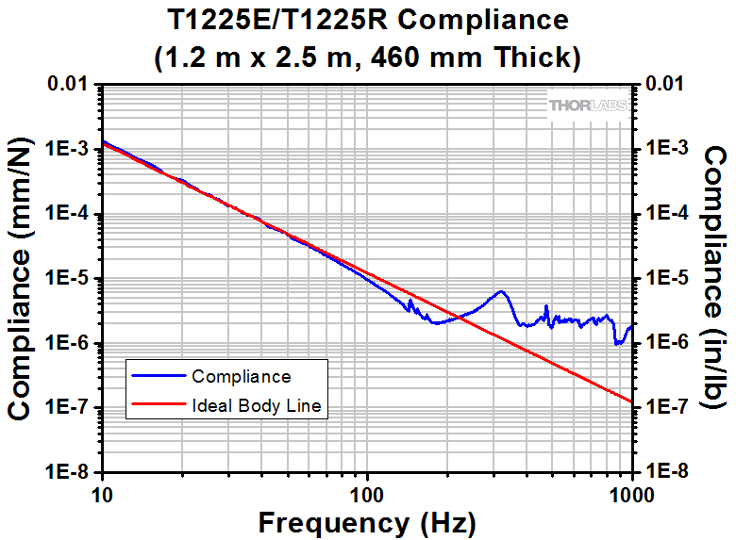
\includegraphics[width=12cm]{Pictures/OpticalTableCompliance}
\caption[Diagram of the Compliance Curve of the Thorlabs T1225E Optical Table]{Diagram of the Compliance Curve of the Thorlabs T1225E Optical Table\cite{ThorlabsComplianceOpticalTable}}
\label{OpticalTableCompliance}
\end{center}
\end{figure}

Optical tables are usually classified by their rigidity as well as their dampening capability. It is especially important to not only consider the rigidity of the table for static load cases, but also for dynamic loads. The data from tests with both load scenarios is shown as a so called "Compliance Curve". In figure \ref{OpticalTableCompliance} the Compliance Curve of the optical table used for the the setup of the Artificial Eye is shown. The X axis is showing the Frequency in Herz (hz) in which load was applied to the table. The Y axis on the left shows the relative deformation of the optical table in [mm/N]. This deformation was taken with a located 150 mm from the corner of the table top. The Y axis on the right hand side shows the same deformation in [in/lb].\cite{LoefflerLang2020}\cite{ThorlabsComplianceOpticalTable}


\section{Network}
In order to have a fast and reliable communication between the cameras, the spectrometer and the computer, the network settings for all network participants needed to be configured correctly. 

\subsection{Configuration Cameras}
First, the cameras should be configured. On default, the cameras are set to DHCP. This means that their IP-address will be automatically changed in order to communicate with the PC. This makes it easy to find them as long as the PC network card is configured in the same way, which it is by default. The network setting of the Lucid cameras can be configured via the network configuration "ArenaConfig" tool provided by Lucid. It is located in the root directory of the camera software "ArenaView". With this tool, the IP-address of the cameras could be configured to be persistent (not automatically changing). This is done in order to enable programs like LabVIEW to find the cameras always on the same IP-address. Currently, the cameras are set to an IP-address range from 10.10.10.2 - 10.10.10.5. The configuration is shown in figure \ref{AppIPcam}.

\subsection{Configuration network card}
Second, the network card of the PC will be configured. Here, two important settings needed to be changed in order to establish a fast and reliable connection to the devices in the lab. First, the IP-address of the PC itself needed to be changed. This could be done under the tab "change adaptor settings" in the network configurations of windows. The current network configuration is shown in figure \ref{AppIPpc}.\\
The second important setting is called "Jumbo packets". It can be found in the same location as the settings for the IP and enables devices like the cameras to send bigger data packets. This is very important in order to read the data from all cameras in the least amount of time possible. The correct configuration is shown in figure \ref{AppJumbo}.

\begin{figure}
\begin{center}
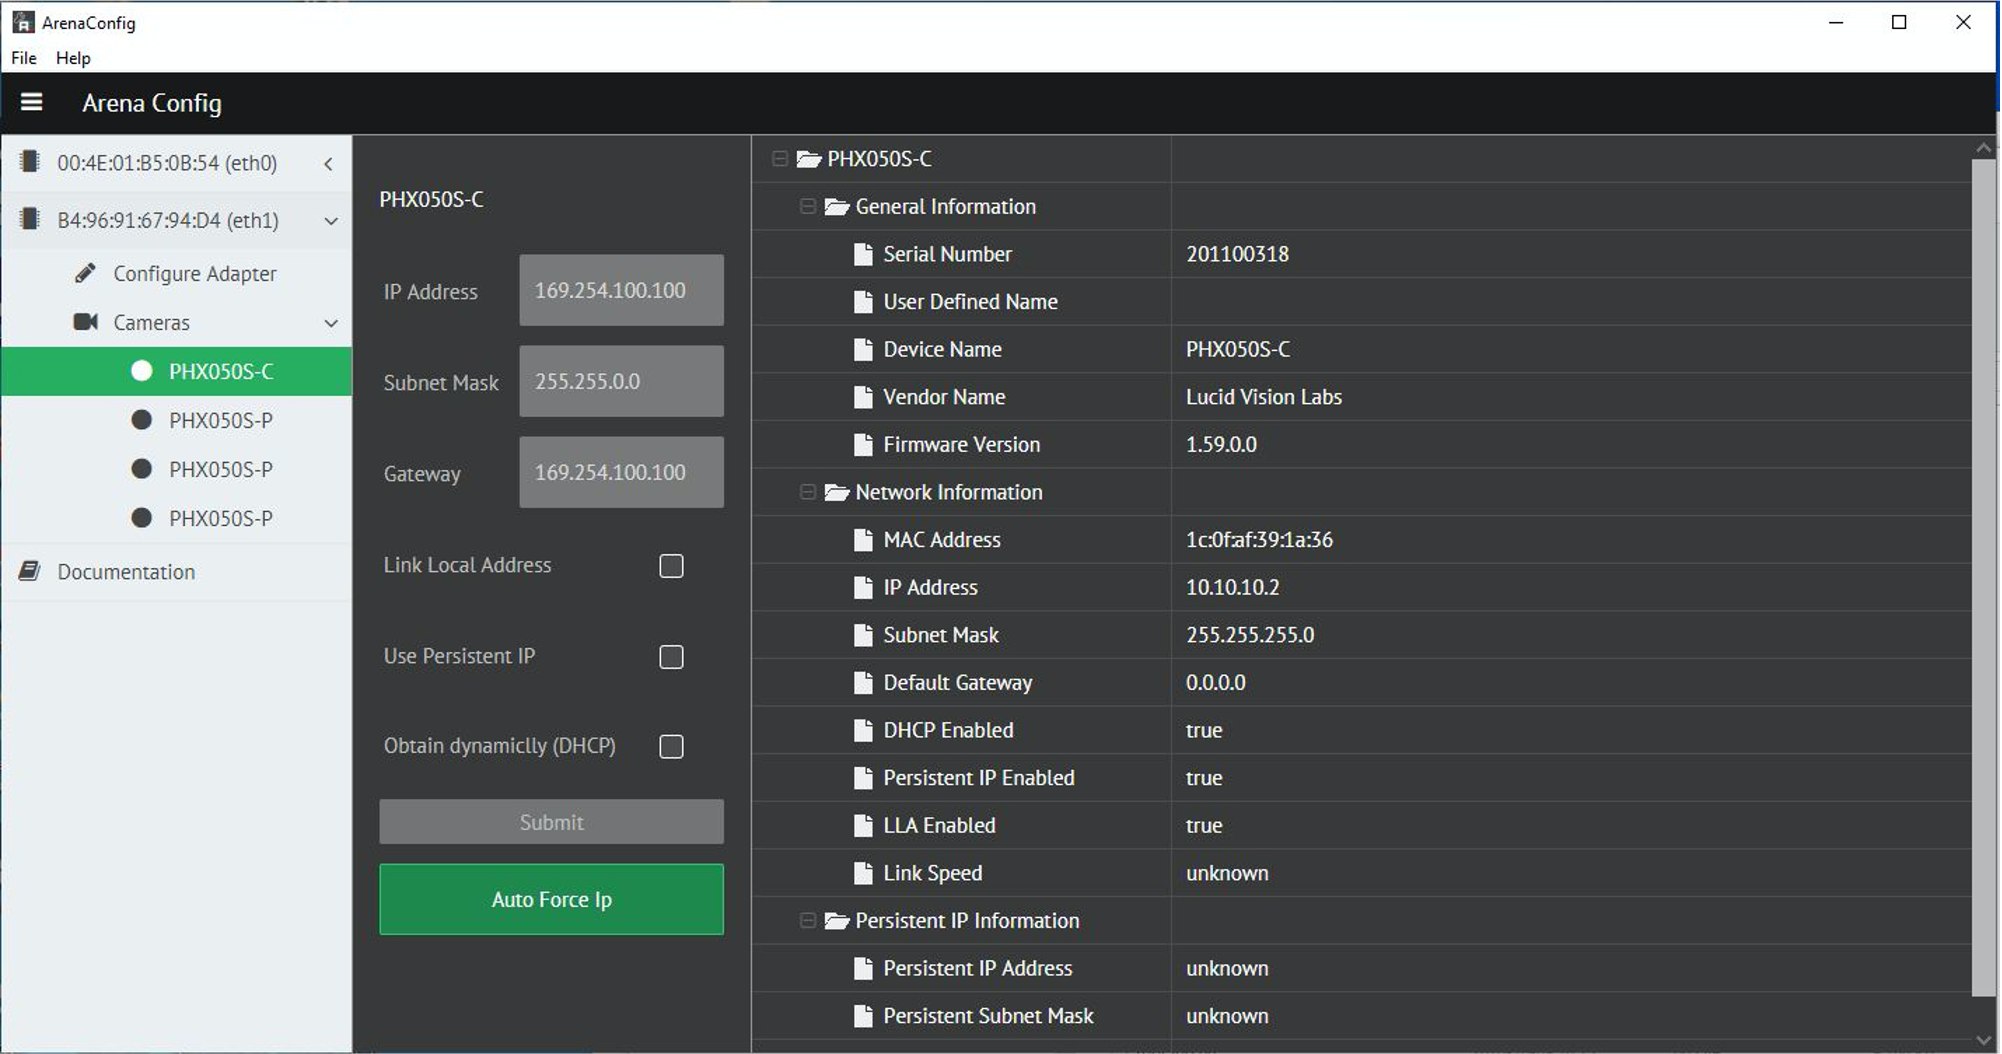
\includegraphics[width=12cm]{Pictures/AppIPcam}
\caption[Picture of the network settings for the RGB camera]{Picture of the network settings for the RGB camera: Red bordered - Network configuration}
\label{AppIPcam}
\end{center}
\end{figure}

\begin{figure}
\begin{center}
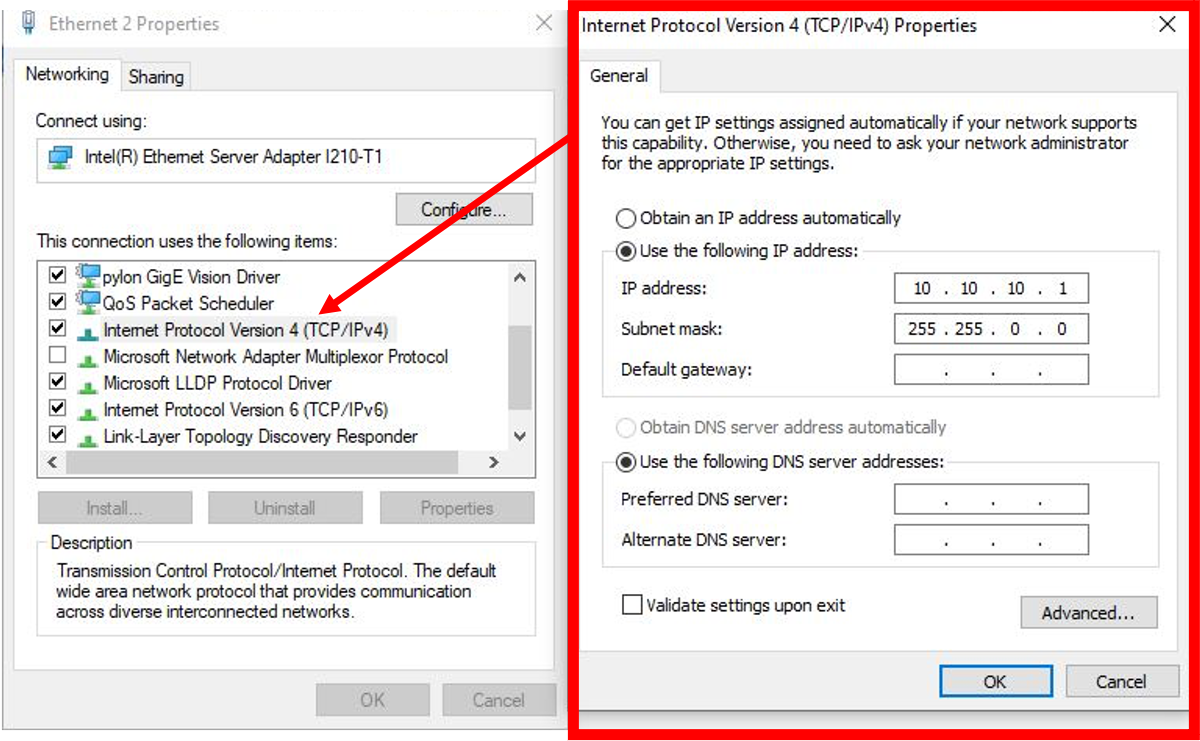
\includegraphics[width=12cm]{Pictures/AppIPpc}
\caption[Picture of IP settings for the network card of the PC]{Picture of IP settings for the network card of the PC: Red bordered - IPV4 protocol settings}
\label{AppIPpc}
\end{center}
\end{figure}

\begin{figure}
\begin{center}
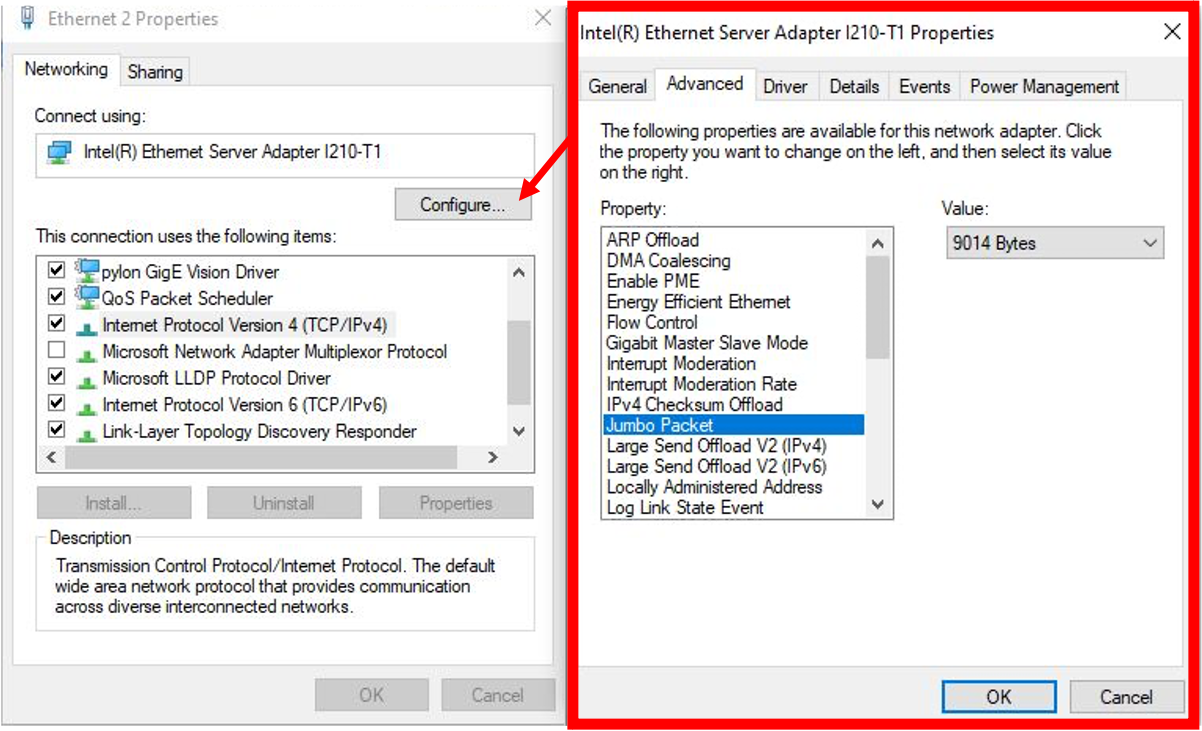
\includegraphics[width=12cm]{Pictures/AppJumbo}
\caption[Picture of Jumbo packet settings]{Picture of Jumbo packet settings: Red bordered - Jumbo packet settings}
\label{AppJumbo}
\end{center}
\end{figure}













